 % http://www.risc.jku.at/people/ckoutsch/stuff/e_algorithms.html
 
 
 \begin{textarea}[]
 	\only<1>{
 		Algorithm that solves the single-source shortest path problem for a directed graph with nonnegative edge weights. 
 	}
 	\only<2>{
 		What is Dijkstra's algorithm.
 	}
 \end{textarea}

\begin{textarea}[]
	\only<1>{
		Technique for finding a particular value in a linear array by ruling out half of the data at each step.
	}
	\only<2>{
		What is Binary Search.
	}
\end{textarea}


\begin{textarea}[]
	\only<1>{	
	%\includemovie{5cm}{5cm}{media/Merge-sort-example-300px.gif}
	\animategraphics{80}{categories/media/Merge-}{0}{211}
	}
	\only<2>{
		What is Mergesort.
	}
\end{textarea}


\begin{textarea}[]
	\only<1>{	
		This algorithm gets you from the time domain to the frequency domain.
		
		P.S.: It's FAST!
	}
	\only<2>{
		What is the FFT.
	}
\end{textarea}

\begin{textarea}[]
  \only<1>{
    \begin{algorithm}[H]
      \begin{algorithmic}[1]
        \FOR {$k = 1 \cdots n$}
        \FOR {$i = k+1 \cdots n$}
        \STATE $m := A[i, k] / A[k, k]$
        \FOR {$j = k+1 \cdots n$}
        \STATE $A[i, j]  := A[i, j] - A[k, j] * m$
      \ENDFOR
      \STATE $A[i, k]  := 0$
    \ENDFOR
  \ENDFOR
\end{algorithmic}
\end{algorithm}
}
\only<2>{
  What is the Gauss-Algorithm?
}
\end{textarea}

% 100
\begin{textarea}[]
  \only<1>{
    \begin{algorithm}[H]
      \textbf{FUNCTION} blublub(A)
      \begin{algorithmic}[1]
        \FOR {$n = size(A) \cdots 2$}
        \FOR {$i = 0 \cdots n-2$}
        \IF {$A[i] > A[i+1]$}
        \STATE Swap$(A[i],A[i+1])$ 
      \ENDIF
    \ENDFOR
  \ENDFOR
\end{algorithmic}
\end{algorithm}
}
\only<2>{
  What is Bubble Sort?
}
\end{textarea}

%200
\begin{textarea}[]
  \only<1>{
    \begin{algorithm}[H]
      \begin{algorithmic}[1]
        \WHILE {$\vert df \vert > \varepsilon $}
        \STATE $df = \text{gradientF(x)}$
        \STATE $x = x-\alpha df$
      \ENDWHILE
    \end{algorithmic}
  \end{algorithm}
}
\only<2>{
  What is Steepest Descent?
}
\end{textarea}

\begin{textarea}[]
  \only<1>{
    \centering
    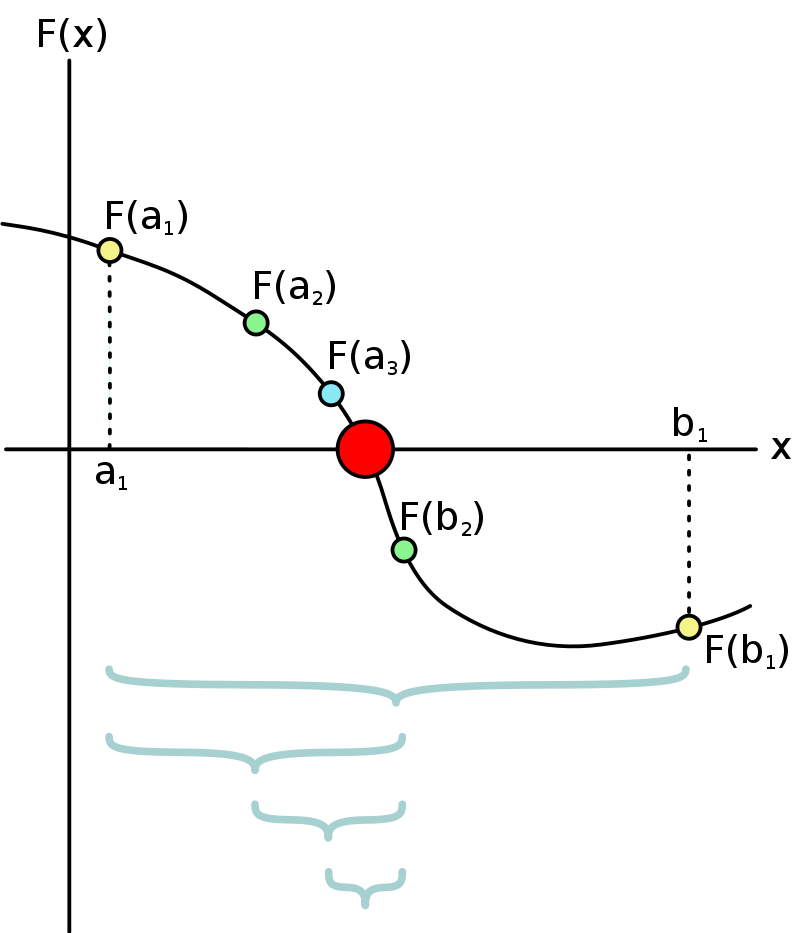
\includegraphics[height=0.5\linewidth]{categories/media/800px-Bisection_method}
  }
  \only<2>{
    What is the Bisection Algorithm?
  }
\end{textarea}

\begin{textarea}[]
  \only<1>{
    \centering
    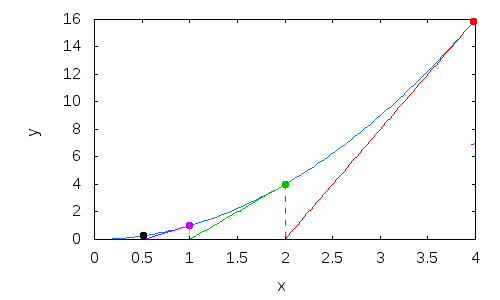
\includegraphics[height=0.5\linewidth]{categories/media/Newtons_method_x2}
  }
  \only<2>{
    What is Newton's method?
  }
\end{textarea}





\begin{textarea}[]
	\only<1>{
		\begin{algorithm}[H]
			\textbf{FUNCTION} F(n)
			\begin{algorithmic}[1]
				\IF{$n \leq 1$}
				\RETURN $n$
				\ELSE
				\RETURN $F(n-1)+F(n-2)$
				\ENDIF
			\end{algorithmic}
		\end{algorithm}
	}
	\only<2>{
		What is the Fibonacci Algorithm?
	}
\end{textarea}







% % % % % % % % % % % % % % % % % % % % % % % % % % % % %


\begin{textarea}[]
	\only<1>{
		\begin{algorithm}[H]
			\begin{algorithmic}[1]
				\STATE n = length(A)
				\WHILE{ true}
				\STATE swapped = false
				\FOR{$i=1...n-1$}
				\IF {$A[i-1] > A[i]$ }
				\STATE swap( A[i-1], A[i] )
				\STATE swapped = true
				\ENDIF
				\ENDFOR
				\IF{not swapped}
				\RETURN
				\ENDIF
				\ENDWHILE
			\end{algorithmic}
		\end{algorithm}
	}
	\only<2>{
		What is the Bubblesort?
	}
\end{textarea}
